% !TeX document-id = {e03e7fd2-79d7-4ae2-923d-792ccfc7ca6e}
% !TeX TS-program = lualatex
% !BIB TS-program = biber

\documentclass[12pt,openany]{book}

\usepackage{iftex}

\ifPDFTeX
	\usepackage{cmap} % should be first
	\usepackage[utf8]{inputenc}
	\usepackage[T1,T2A]{fontenc}
	\usepackage[english,russian]{babel}

	\usepackage[breakwords]{truncate}
\fi

\ifLuaTeX
	\usepackage{fontspec}

	% from https://github.com/AndreyAkinshin/Russian-Phd-LaTeX-Dissertation-Template/
	\setmonofont{CMU Typewriter Text}
	\newfontfamily\cyrillicfonttt{CMU Typewriter Text}
	\defaultfontfeatures{Ligatures=TeX}
	\setmainfont{CMU Serif}
	\newfontfamily\cyrillicfont{CMU Serif}
	\setsansfont{CMU Sans Serif}
	\newfontfamily\cyrillicfontsf{CMU Sans Serif}
	
	\usepackage{polyglossia}
	\setmainlanguage[babelshorthands=true]{russian}
	\setotherlanguage{english}
%	\setotherlanguage{german}
	
	\usepackage[fit]{lualatex-truncate}
\fi

% Programming
\usepackage{xifthen}

% Language support

\usepackage{csquotes}

% Typesetting
\usepackage{enumitem}
\usepackage{indentfirst}
\usepackage{titlesec}
%\usepackage{tocbibind}
\usepackage{xspace}
\usepackage{setspace}
\onehalfspacing

% Extra symbols
\usepackage{fontawesome5}
\usepackage{textcomp}

% Tables
\usepackage{array}
\usepackage{booktabs}

% Highlightiing
\usepackage[normalem]{ulem}

% Math
\usepackage{amsmath}
\usepackage{amssymb}
\usepackage{commath}
\newcommand{\vect}[1]{\mathbf{#1}}
\DeclareMathOperator{\const}{const}




%%% Drawing with TikZ / pgfplots
\usepackage{graphicx}

\usepackage[svgnames,x11names]{xcolor}
\colorlet{tabblue}{blue!70!green}
\colorlet{tabgreen}{green!50!black!85!white}
\colorlet{taborange}{orange}
\colorlet{tabred}{red!80!black}

\usepackage{tikz}
\usetikzlibrary{arrows.meta}
\usetikzlibrary{bbox}
\usetikzlibrary{calc}
\usetikzlibrary{decorations.markings}
\usetikzlibrary{decorations.pathmorphing}
\usetikzlibrary{decorations.pathreplacing}
\usetikzlibrary{external}
\usetikzlibrary{fadings}
\usetikzlibrary{math}
\usetikzlibrary{matrix}
\usetikzlibrary{patterns}
\usetikzlibrary{positioning}
\usetikzlibrary{shapes.geometric}
\usetikzlibrary{shapes.misc}


%%% PGFplots setup
\usepackage{pgfplots}
\usepackage{pgfplotstable}

\newcommand{\tickprint}[1]{\small\pgfmathprintnumber[verbatim,#1]{\tick}}

\pgfplotsset{
	compat=newest,
	xticklabel=\tickprint{},
	yticklabel=\tickprint{},
	scaled y ticks=false,
	%	set layers=axis on top, % BAD!
	every axis/.append style={
		line width=0.6pt, % /tikz/semithick==0.6pt
		%
		scaled y ticks=false,
		ticklabel shift=0pt,
		tick align=inside,
		tick pos=left,
		tickwidth=0.6pt,
		subtickwidth=0.6pt,
		major tick length=3pt,
		minor tick length=1.5pt,
		tick style={semithick,black,overlay},
		%
		minor tick num=4,
	},
}






%%% TikZ helpers (for debug purposes)
\tikzset{nosep/.style={inner sep=0,outer sep=0}}

\newcommand{\helpangles}[1]{
	\foreach \a in {0,5,...,355} \draw[help lines] (#1.center) -- (#1.\a) -- ++(\a:0.5) node[font=\tiny] {\a};
}

\tikzset{%
	show curve controls/.style={
		postaction={
			decoration={
				show path construction,
				curveto code={
					\draw [blue,very thin]
					(\tikzinputsegmentfirst) -- (\tikzinputsegmentsupporta)
					(\tikzinputsegmentlast) -- (\tikzinputsegmentsupportb);
					\fill [red, opacity=0.5]
					(\tikzinputsegmentsupporta) circle [radius=.5ex]
					(\tikzinputsegmentsupportb) circle [radius=.5ex];
				}
			},
			decorate
}}}
\tikzset{show curve controls/.style={}}  % disables code above




% Hyperlinks
\usepackage{hyperref}  % should be last
\hypersetup{
	linktocpage,
	colorlinks,
	linkcolor={red!70!black},
	citecolor={green!50!black},
	urlcolor={blue!80!black}
}
\newcommand*{\email}[1]{\href{mailto:#1}{\nolinkurl{#1}} } 


%%% Colorful fixmes and missing refs and missing cites (if no biblatex is present)
% !TeX root = phd_thesis_Syromyatnikov.tex

% MUST GO AFTER \usepackage{hyperref}

% makes fixes colorful
\usepackage{fixme}
\usepackage{soulutf8}
\usepackage{etoolbox}

\ifLuaTeX
	% https://tex.stackexchange.com/questions/339382/soul-highlight-removes-some-characters-from-text
	\makeatletter
	\font\SOUL@tt="CMU Typewriter Text"
	\setbox\z@\hbox{\SOUL@tt-}
	\SOUL@ttwidth\wd\z@ %reset default width of -
	\makeatother
\fi

\fxsetup{status=draft,author= ,layout=inline,nomargin,theme=color}
\definecolor{fxnote}{rgb}{0,0,0}
\definecolor{fxwarning}{rgb}{0,0,0}
\definecolor{fxerror}{rgb}{0,0,0}
\definecolor{fxfatal}{rgb}{0,0,0}

\colorlet{fxnotebg}{green!60}
\colorlet{fxwarningbg}{yellow!60}
\colorlet{fxerrorbg}{red!40!orange!50}
\colorlet{fxfatalbg}{red!70}
% redefine the layout macro:
\makeatletter
\renewcommand*\FXLayoutInline[3]{%
    \@fxdocolon {#3}{%
        \@fxuseface {inline}%
        \begingroup
        \sethlcolor{fx#1bg}%
        \color{fx#1}\ignorespaces \hl{#3\@fxcolon #2}%
        \endgroup}}

\renewcommand*\FXLayoutContentsLine[3]{%
    \iffx@mode@multiuser%
    \fxaddcontentsline{\ignorespaces#3 \protect\sethlcolor{fx#1bg}\color{fx#1}\hl{\fxnotename{#1}:\thesection #2}}%
    \else%
    \fxaddcontentsline{\protect\sethlcolor{fx#1bg}\color{fx#1}\hl{%
    	\fxnotename{#1}:~\texttt{\thesection}~#2%
    }}%
    \fi}
\makeatother


% emphasizes missing references and citations
\makeatletter
\patchcmd{\@setref}{\bfseries ??}{\fxerror{Ref}}{}{}
\patchcmd{\@citex}{\bfseries ?}{\fxerror{Cite}}{}{}
\patchcmd{\NAT@citexnum}{\reset@font\bfseries?}{\fxerror{Cite}}{}{}
\patchcmd{\NAT@citex}{\reset@font\bfseries ?}{\fxerror{Cite}}{}{}
\makeatother
  % must go after hyperref




%%% Bibliography
\usepackage[backend=biber,
clearlang=true,autolang=other,language=autobib,
style=nature,
doi=false,url=false,eprint=false,isbn=false,
sorting=none,sortcites=true,
maxnames=7,minnames=3,defernumbers=true,date=year]{biblatex}

\addbibresource{bib/litreview.bib}
\addbibresource{bib/methods.bib}
\addbibresource{bib/interaction.bib}
\addbibresource{bib/formation.bib}
\addbibresource{bib/eqnoneq.bib}
\addbibresource{bib/spt.bib}

\addbibresource{bib/2020-review.bib}
\addbibresource{bib/master-diploma.bib}

\addbibresource{bib/articles.bib}
\addbibresource{bib/conferences.bib}

\AtEveryBibitem{
	\clearfield{issn}
	\clearfield{issue}
	\clearfield{month}
	\clearfield{abstract}
	\clearlist{language}
}

%\renewcommand{\finalnamedelim}{\addcomma\space\bibstring{and}\space}
\renewcommand{\finalnamedelim}{\addcomma\space}

\renewcommand{\bibrangedash}{\textendash}


%%% Git version
\usepackage{shellesc}
%\ShellEscape{git describe --tags --always --abbrev=40 --dirty > git-version.tex}
\ShellEscape{git describe --always --abbrev=40 --always > git-version-commit.tex}
\ShellEscape{git describe --tags --abbrev=10 --always > git-describe.tex}

\usepackage{catchfile}
%\CatchFileDef{\GitVersion}{git-version.tex}{}
\CatchFileDef{\GitCommit}{git-version-commit.tex}{}
\CatchFileDef{\GitDescribe}{git-describe.tex}{}
\hypersetup{pdfinfo={GitVersion={\GitDescribe},GitCommit={\GitCommit}}}
\usepackage[useregional]{datetime2}




%%% Technical stuff
\usepackage[figure,table,xspace]{totalcount} % count figures and tables

\usepackage{lastpage} % count pages
\usepackage{refcount}

\usepackage{totcount} % count bibliography items
\newtotcounter{phdthesiscitenum}
\setcounter{phdthesiscitenum}{-21} 
% 21 = 10 articles + 11 abstracts
\AtEveryBibitem{\stepcounter{phdthesiscitenum}}

\usepackage{lipsum}


%%% Footnote without number
\newcommand\blindfootnote[1]{%
	\begingroup
	\renewcommand\thefootnote{}\footnote{#1}%
	\addtocounter{footnote}{-1}%
	\endgroup
}


%%% Further tweaking
\renewcommand{\arraystretch}{1.2} % more vertical space in tables

% \overfullrule=2mm % shows overfull markers without 'draft' option


\usepackage[%
	a4paper, asymmetric,
	top=2cm, bottom=3cm, left=2.5cm, right=2cm,
]{geometry}

\usepackage{fixme} % imported again because of TeXStudio doesn't want highlight notes

\tikzexternalize[prefix=tikzfigures/] % we want different folders for thesis and autoreferat

%%% Page headers / footers
\usepackage{fancyhdr}
\pagestyle{fancy}
\setlength{\headheight}{15.5pt} % fixes fancyhdr warning
\renewcommand{\chaptermark}[1]{\markboth{\scshape\chaptername~$\thechapter$.~\truncate{0.4\linewidth}{#1}}{}}
\renewcommand{\sectionmark}[1]{\markright{\slshape\thesection.~\truncate{0.4\linewidth}{#1}}}

\fancyhead[R]{\rightmark}
\fancyhead[L]{\leftmark}
\fancyfoot[C]{\thepage}
\renewcommand{\headrulewidth}{0.4pt}
\renewcommand{\footrulewidth}{0pt}

%%% strip all figures
%\usepackage{environ}
%\RenewEnviron{figure}{}

%%% show all keys
%\usepackage{showkeys}

\begin{document} %%%%%%%%%%%%%%%%%%%%%%%%%%%%%%%%%%%%%%%%%%%%%%%%%%%%%%%%%%%%%%%%%%%%%%%%%%%%%%%%%%%%%%%%%%%%

% !TeX root = phd_thesis_Syromyatnikov.tex

\newcommand{\thisyear}{2020}
\newcommand{\HRule}{\rule{\linewidth}{0.3mm}}

\begin{titlepage}
\begin{center}
%\textsc{\Large Федеральное государственное бюджетное образовательное учреждение высшего образования}\\
\textsc{\Large Московский государственный университет имени М.~В.~Ломоносова \\[0.27cm] Физический факультет}\\
\vspace{2cm}

\hfill на правах рукописи \\
\vspace{1.8cm}

\textbf{\Large Сыромятников Алексей Геральдович}
\vspace{1cm}

\HRule 
\vspace{0.4cm}
\begin{spacing}{1.6}
\textbf{\huge Теоретическое исследование процессов формирования и структурных свойств металлических атомных проводов}
\end{spacing}
\vspace*{0cm}
\HRule 
\vspace{1cm}

Специальность \texttt{01.04.07} --- физика конденсированного состояния
\vspace{1cm}

{\large Диссертация на соискание учёной степени кандидата физико-математических наук}
\end{center}

\vspace{1cm}
\hfill
\begin{minipage}[t]{0.65\textwidth}
	\begin{flushright} \large
	Научный руководитель: \\
	кандидат физико-математических наук, доцент \\
	\textsc{Клавсюк} Андрей Леонидович
	\end{flushright}
\end{minipage}


%----------------------------------------------------------------------------------------
%	DATE SECTION
%----------------------------------------------------------------------------------------

\vfill
\begin{center}
\large Москва --- \thisyear
\end{center}
\end{titlepage}



\pagenumbering{Roman}

%\listoffixmes\vspace*{1cm}
%\input{TODO}

\tableofcontents

%\setstretch{1.3}
\clearpage
\pagenumbering{arabic}

\fancyhead[R]{}
\fancyhead[L]{\scshape Введение}

% Введение
\chapter*{Введение}
\addcontentsline{toc}{chapter}{Введение}
\label{chap:introduction}

\newcommand{\psection}[1]{\vspace*{0.3cm}\textsc{\bfseries{#1}}\par}
\newcommand{\compenspace}{\vspace*{-0.3cm}}

\compenspace

\psection{Актуальность темы}
Научно-технологический прогресс в настоящее время неотделим от постоянной миниатюризации различных электронных устройств, в частности интегральных микросхем и элементов памяти.
Новейшие устройства такого типа строятся на базе наноразмерных электронных компонентов, среди которых транзисторы, цепочки и провода.
Характерные линейные размеры таких объектов сегодня приближаются к единицам нанометров. Оперировать атомными структурами такого размера очень трудно, поэтому прикладные и фундаментальные исследования в этой области сейчас актуальны как никогда.

Помимо этого одномерные наноструктуры обладают рядом уникальных свойств, среди которых волны спиновой и зарядовой плотности~\cite{Erwin2010}, квантованная проводимость~\cite{Klavsyuk2015}, эффект Рашбы~\cite{Rasba84.1}.
Свойства таких одномерных структур существенно отличаются как от свойств объемного образца, так и от свойств тонких пленок и квантовых точек.
Создание наноразмерных структур на текущий момент возможно либо при помощи литографических методов, либо путем перетаскивания отдельных атомов иглой сканирующего туннельного микроскопа.
Оба подхода имеют свои недостатки, не позволяющие получать такие одномерные наноструктуры в промышленных масштабах.
Ситуация может измениться с использованием метода самоорганизации наноструктур путем эпитаксиального роста.
Однако для того чтобы использование наноструктур в промышленности стало реальностью, необходимо уметь управлять их созданием, что невозможно без понимания механизмов, ответственных за их рост.

В связи с этим особенно актуальны исследования структурных, электронных и магнитных свойств наноструктур на поверхности металлов, а также установление закономерностей в их росте и эволюции.


\psection{Цель и задачи работы}
Основной целью диссертационной работы являются исследование механизмов роста атомных структур на поверхности металлов и установление особенностей их атомной структуры с использованием современных теоретических методов. Исследование механизмов роста включает в себя не только моделирование процессов самоорганизации, но и исследование взаимодействия атомов $3d$-металлов на поверхностях металлов. Для достижения поставленной цели решались следующие задачи:
\begin{enumerate}
	\item Разработать методику теоретического исследования и моделирования  формирования и дальнейшей эволюции одномерных атомных структур на поверхности металлов.
	\item Исследовать взаимодействие адатомов $3d$-металлов со ступенью вицинальной поверхности меди.
	\item Определить превалирующие факторы, влияющие на рост одномерных наноструктур на вицинальных металлических поверхностях.
	\item Показать зависимость формы распределения длин атомных цепочек от параметров эксперимента.
	\item Создать модель, описывающую распределение одномерных атомных структур, учитывающую созревание Оствальда и распад коротких одномерных структур.
	\item Исследовать структурный фазовый переход из димеризованного в недимеризованное состояние у атомных цепочек кобальта.
\end{enumerate}

Поставленные задачи важны как с фундаментальной, так и с практической точки зрения.

\psection{Научная новизна работы}

В диссертационной работе получены следующие научные результаты:
\begin{enumerate}
	\item На основе метода Монте-Карло разработана методика численного моделирования формирования и эволюции морфологии одномерных металлических структур на вицинальных металлических поверхностях, а также исследован структурный фазовый переход в них.
	\item Определены особенности взаимодействия адатомов $3d$-металлов со ступенью вицинальной поверхности меди и объяснена их природа. Установлена зависимость взаимодействия между двумя адатомами $3d$-металлов на вицинальной поверхности меди от расстояния до ступени.
	\item Впервые исследован рост и последующая эволюция одномерных атомных структур при двухтемпературном режиме.
	\item Выявлена зависимость формы распределения длин атомных цепочек от таких параметров эксперимента, как температура, поток напыляемых атомов, степень покрытия.
	\item Впервые предложен метод более точного определения значения энергии связи в одномерных атомных структурах.
	\item Установлена зависимость температуры структурного фазового перехода от длины цепочки  и от энергии димеризации.
\end{enumerate}




\psection{Научная и практическая значимость работы}
Полученные результаты могут иметь важное значение в решении прикладных задач по созданию новых методик производства элементов памяти и передачи информации в промышленности. Кроме того, модели описания роста одномерных структур необходимы для более корректного анализа экспериментальных данных.

Работа была  выполнена при финансовой поддержке Российского Фонда Фундаментальных Исследований (гранты 19-32-90045, 19-12-50010) и Фонда развития теоретической физики и математики ``БАЗИС''. При выполнении работы были использованы вычислительные ресурсы Научно-исследовательского вычислительного центра Московского государственного университета им. М.~В.~Ломоносова (НИВЦ МГУ).


\psection{Положения, выносимые на защиту}
\begin{enumerate}
	\item Метод моделирования формирования и эволюции одномерных структур на вицинальных металлических поверхностях.
	\item Микроскопический механизм формирования металлических атомных проводов на вицинальных металлических поверхностях, сценарии эволюции системы атомов при различных внешних условиях.
	\item Модель для описания распределения одномерных атомных структур, в рамках которой возможно более точное определение значения энергии связи.
	\item Структурный фазовый переход в атомных проводах Co на поверхности Cu(775).
\end{enumerate}

\psection{Достоверность результатов}
Результаты, представленные в диссертационной работе, получены с использованием  современных методов теоретической физики. Обоснованность и достоверность определяются адекватностью применяемых моделей и сравнением с экспериментальными данными.

\psection{Апробация результатов}
Основные результаты диссертации были представлены автором лично на следующих мероприятиях:
\begin{itemize}[nosep]
	\item VIII Всероссийская научная молодежная школа-конференция ``Химия, физика, биология: пути интеграции'' (Москва, Россия, 2020);
	\item 8-ая Международная мастерская по магнитным проводам IWMW-2019 (Светлогорск, Россия, 2019);
	\item III Международная Балтийская конференция по магнетизму IBCM-2019 (Светлогорск, Россия, 2019);
	\item Международная конференция по нанонауке и технологии ICN+T (Брно, Чехия, 2018);
	\item VI Научная молодежная школа-конференция ``Химия, физика, биология: пути интеграции'' (Москва, Россия, 2018);
	\item V Научная молодежная школа-конференция ``Химия, физика, биология: пути интеграции'' (с. Ершово, Московская обл., Россия, 2017);
	\item 32-я Европейская конференция физики поверхности ECOSS-32 (Гренобль, Франция, 2016);
	\item 23-я Международная научная конференция студентов, аспирантов и молодых ученых ``Ломоносов-2016'' (Москва, Россия, 2016);
	\item 22-я Международная научная конференция студентов, аспирантов и молодых ученых ``Ломоносов-2015'' (Москва, Россия, 2015);
\end{itemize}

\psection{Публикации}
По теме диссертации опубликовано 10 научных статей и тезисы к 11 докладам на научных конференциях (всего 21 печатная работа).

\psection{Личный вклад автора}
Вклад автора в диссертационную работу является определяющим. Все основные результаты работы получены автором лично, либо при его непосредственном участии.

\psection{Структура и содержание работы}
Диссертация состоит из введения, шести глав, заключения и списка литературы.
Работа изложена на \getrefbykeydefault{LastPage}{page}{0}~страницах, включает \totalfigures~рисунка и \totaltables~таблицы. Общее число ссылок составляет \total{phdthesiscitenum}.
Каждую главу предваряет вступительная часть, представляющая краткое содержание и основные задачи текущей главы.
В конце диссертации сформулированы основные результаты, достигнутые в ней.


\clearpage
\fancyhead[R]{\rightmark}
\fancyhead[L]{\leftmark}

% Литобзор
% !TeX root = phd_thesis_Syromyatnikov.tex

\chapter{Исследование формирования и структурных свойств наноструктур Co на вицинальной поверхности меди (111) (обзор литературы)}

Исследование физики и химии поверхности твердого тела в условиях сверхвысокого вакуума производится в течение уже очень долгого времени~\cite{Giesen2001}. Для этого применяют самые разнообразные методы~\cite{Oura2006}. Например, спектроскопические методы, среди которых спектроскопия характеристических потерь энергии электронами~\cite{Ibach1994,Ibach1991}, фотоэлектронная и инфракрасная спектроскопия~\cite{Greenler1966,Bradshaw1969,DUMAS1999}, которые позволяют получить информацию о химии поверхности и кинетике реакций на ней. Детальное изучение структуры поверхности стало возможным благодаря сканирующей и отражательной электронной микроскопии~\cite{Bauer1994,Bauer1994a}, а также сканирующей туннельной микроскопии~\cite{Binnig1982} (СТМ) и другим сканирующим зондовым методам, таким как атомная силовая микроскопия (АСМ)~\cite{PhysRevLett.56.930}.

Важным элементом поверхности твердого тела являются ее дефекты. Они выступают в роли предпочитаемых мест реакции или прикрепления химически либо физически адсорбированных атомов и молекул. Чтобы иметь представление о кинетике поверхностных дефектов, необходимо иметь информацию о локальном строении поверхности.

Первой вехой в изучении локальной атомной структуры поверхностей и кинетики адатомов на ней в условиях сверхвысокого вакуума стал полевой ионный микроскоп~\cite{Mller1951} (ПИМ), ставший развитием идей, заложенных полевой электронной микроскопией~\cite{Mller1937}. ПИМ способен проводить прямые наблюдения свободных адатомов на острой металлической игле.
Дифракционные методы, среди которых отражательная и низкоэнергетическая электронная микроскопия~\cite{Bauer1994,Bauer1994a}, не ограничены небольшим рядом материалов, в отличие от ПИМ.

Прорывом в изучении локальной атомной структуры поверхности и, в частности, локальных дефектов и их кинетики в ультравысоком вакууме стало применение СТМ\cite{Binnig1982,PhysRevLett.49.57,PhysRevLett.50.120}.
Ранние версии СТМ могли работать только при комнатной температуре, а небольшие колебания температуры во время эксперимента существенно изменяли получаемые данные из-за теплового расширения иглы и остальных компонентов микроскопа.
Появившиеся позже низкотемпературные СТМ~\cite{denHaan2014}, демонстрирующие очень низкий температурный дрейф, можно выделить в отдельный класс экспериментальной аппаратуры. Отдельным преимуществом низкотемпературных исследований является тот факт, что при низкой температуре граница между занятыми и незанятыми электронными состояниями проявляется очень резко, что используется в сверхчувствительной спектроскопии~\cite{Song2010}.
В зависимости от температуры и от изучаемого образца, скорость поверхностной диффузии может быть либо ниже, либо выше скорости получения СТМ изображения. В первом случае отдельные СТМ изображения представляют собой снимки структуры поверхности. Движение атомов и таких дефектов поверхности, как кинки или ступени, может быть изучено путем анализа изменений в последовательных СТМ изображениях. На сегодняшний день высокоскоростной СТМ позволяет наблюдать образец с частотой более 100 кадров в секунду в условиях постоянно меняющейся температуры~\cite{Frenken2017}. Однако во втором случае поверхность изменяется во время записи одного изображения и даже между последовательными линиями сканирования --- изображения несут в себе уже не только пространственную информацию, но и временную. Таким образом, информация о процессах диффузии атомов может быть извлечена только путем обращения к теоретическим моделям, которые способны связать макроскопические изменения в структуре поверхности с отдельными атомными процессами.


\section{Вицинальные поверхности (111) и дефекты на них}

\dots



% Постановка задачи
%\input{goal}

% Методы
% !TeX root = phd_thesis_Syromyatnikov.tex

\chapter{ Методы моделирования роста одномерных атомных структур и исследования их структурных свойств}

Для определения атомной структуры на поверхности металлов существует много различных методов. Сюда относятся, в порядке уменьшения точности: ``первопринципные'' методы, метод молекулярной динамики (МД), использующий полуэмпирические потенциалы, методы Монте-Карло. Огромным недостатком ``первопринципных'' методов является их сложность и следующий из неё большой объем вычислений. Метод молекулярной динамики не позволяет исследовать эволюцию систем на больших промежутках времени. Методы Монте-Карло построены на использовании случайных чисел, что позволяет получить статистически точный ответ только по прошествии большого количества шагов.

\begin{figure}
	\centering
	\tikzsetnextfilename{metropolis_scheme}
	\begin{tikzpicture}[scale=3.5]
	\fill[green!30!white] (0,0) -- plot[domain=0:2,smooth,variable=\x] ({\x}, {exp(-\x)}) -- (2,0) -- cycle;
	\fill[red!30!white] (0,1) -- plot[domain=0:2,smooth,variable=\x] ({\x}, {exp(-\x)}) -- (2,1) -- cycle;
	\fill[path fading=west,green!30!white] (0,0) rectangle (-0.5,1);
	\fill[path fading=east,green!30!white] (2,0) -- plot[domain=2:2.2,smooth,variable=\x] ({\x}, {exp(-\x)}) -- (2.2,0) -- cycle;
	\fill[path fading=east,red!30!white] (2,1) -- plot[domain=2:2.2,smooth,variable=\x] ({\x}, {exp(-\x)}) -- (2.2,1) -- cycle;
	
	\draw[-latex] (-0.5,0) -- (2.3,0) node[below right] {$\Delta E$};
	\draw[-latex] (0,0) node[below] {0} -- (0, 1.3) node[below left] {P};
	\node[below left=0 and 0.15] at (0,1) {1};
	\draw (-0.04,1) -- (0.04,1);
	
	\draw[thick] plot[domain=-0.05:2,smooth,variable=\x] ({\x}, {exp(-\x)});
	\node[above right,font=\large] at (1.2,0.3) {$e^{-\frac{\Delta E}{k_BT}}$};
	\end{tikzpicture}
	\caption{Схематическое представление выбора событий в алгоритме Метрополиса. Кривая соответствует функции $\exp \left(-{\Delta E} / {k_BT}\right)$. В зависимости от величины потенциального барьера $\Delta E$, событие либо принимается сразу ($\Delta E<0$) (зеленая зона слева от нуля), либо может быть отброшено с вероятностью $1-P = 1-\exp \left(-{\Delta E} / {k_BT}\right)$ (красная зона над кривой и зеленая зона под кривой справа от нуля). }
	\label{fig:metropolis_scheme}
\end{figure}


\begin{figure}
	\centering
	%	\tikzset{external/force remake}
	\tikzsetnextfilename{kmcChoosing}
	\begin{tikzpicture}
	\tikzmath{\Width = 12;}
	\draw (0,0) rectangle (\Width,1);
	\draw (0.55,0) -- ++(0,1);
	\draw (1.1,0) -- ++(0,1);
	\draw (\Width-0.6,0) -- ++(0,1);
	\node[right] at (0,0.5) {$k_1$};
	\node[right] at (0.55,0.5) {$k_2$};
	\node[left] at (\Width,0.5) {$k_n$};
	
	\tikzmath{\LeftBound = 0.7*\Width; \RightBound = 0.72*\Width;}
	\foreach \x in {1,...,40} \draw ({1.1 + rnd * (\LeftBound - 1.1)}, 0) -- ++(0,1);
	\foreach \x in {1,...,30} \draw ({\RightBound + rnd * (\Width-0.6 - \RightBound)}, 0) -- ++(0,1);
	
	\draw[decorate,decoration={brace,amplitude=5pt,mirror}] (0, -0.1) -- ++(\Width, 0)
	node[midway,below=0.2cm]{$k_{tot}$};
	
	\tikzmath{\Choice = 0.71\Width;}
	\draw[-stealth,very thick] ({1.1 + \Choice * (\Width - 1.1 - 0.6)}, 1.7) -- ++(0,-0.7) node[at start,right] {$r_1 k_{tot}$};
	\draw ({1.1 + \Choice * (\Width - 1.1 - 0.6) - 1}, 1.7) -- ++(1,-1.2) node[at start,left] {$k_q$};
	\end{tikzpicture}
	\caption{Алгоритм случайного выбора состоявшегося события в кинетическом методе Монте-Карло на основании массива частот переходов}
	\label{fig:kmcChoosing}
\end{figure}


\begin{figure}
	\centering
	\tikzset{external/export next=false}
	\begin{tikzpicture}[node distance=0.7cm,bezier bounding box=true]
	\tikzset{
		N/.style={draw,minimum width=4cm,minimum height=1cm,align=left,inner sep=0.5em},
	}
	
	\node[N,shape=chamfered rectangle,minimum width=2cm,fill=red!10] (1) at (0,0) {Начало};
	\node[N,below=of 1] (2) {
		\emph{Инициализация}\\
		Установка параметров расчета\\
		Генерация начального распределения атомов\\
		Распаковка массива потенциальных барьеров
	};
	\node[draw,below=of 2,shape=diamond,align=center,fill=blue!10] (3) {Сделано\\ необходимое\\ число\\ шагов?};
	\node[N,below=1cm of 3] (32) {Построение каталога возможных процессов $\{i \to j\}$};
	\node[N,below=of 32] (4) {Расчет частот $\{k_{ij}\}$~\eqref{eq:transrate}, их суммы $k_{tot}$~\eqref{eq:kmcTotalK}};
	\node[N,below=of 4] (5) {Генерация случайных чисел $r_1$, $r_2$};
	\node[N,below=of 5] (6) {Взвешенный выбор процесса~\eqref{eq:kmcChoose}};
	\node[N,below=of 6] (7) {Реализация выбранного процесса};
	\node[N,below=of 7] (8) {Расчет продолжительности процесса $t_{ij}$~\eqref{eq:kmcHopTime},\\ Обновление таймера};
	\node[N,left=1cm of 3,shape=chamfered rectangle,minimum width=2cm,fill=green!10] (9) {Конец};
	
	\path[->,>=stealth]
	(1) edge (2)
	(2) edge (3)
	(3) edge node[midway,right,red!50!black] {нет} (32)
	(32) edge (4)
	(4) edge (5)
	(5) edge (6)
	(6) edge (7)
	(7) edge (8)
	(8) edge[curve to,out=0,in=0,out looseness=0.5,in looseness=1] (3)
	(3) edge node[midway,above,green!50!black] {да} (9) ;
	\end{tikzpicture}
	\caption{
		Принципиальная схема алгоритма кинетического метода Монте-Карло с априори известными потенциальными барьерами.
	}
	\label{fig:kmcScheme}
\end{figure}


% Основная часть
% !TeX root = phd_thesis_Syromyatnikov.tex

\chapter{Взаимодействие адатомов на вицинальных поверхностях металлов}
\label{chap:interaction}

\blindfootnote{Результаты этой главы были опубликованы в работах A5, A6, A9, A10 из списка публикаций по теме диссертации.}
%\cite{Syromyatnikov:jetp-letters-rus:2014,Syromyatnikov:mplb:2016,Syromyatnikov:PhysRevB:2018, Syromyatnikov:jetp-letters-rus:2018}

\lipsum[1-3]

\section{Раздел 1}
\lipsum[4-7]

\section{Раздел 2}
\lipsum[11-14]

\section{Раздел 3}
\lipsum[6-8]

% !TeX root = phd_thesis_Syromyatnikov.tex

\chapter{Формирование наноструктур на вицинальных поверхностях металлов}
\label{chap:formation}

\blindfootnote{Результаты этой главы были опубликованы в работах A4, A6, A7, A9 из списка публикаций по теме диссертации.}
%\cite{Syromyatnikov:mplb:2016,Syromyatnikov:PhysRevB:2018, SyromyatnikovJetpl2019rus}

\lipsum[1-3]

\section{Раздел 1}
\lipsum[4-7]

\begin{figure}
	\centering
	\tikzsetnextfilename{our_distributions_1T}
	\begin{tikzpicture}
	\pgfplotsset{
		width=0.99\linewidth,
		height=7cm,
		%
		X/.style={mark=none, ultra thick}
	}
	\tikzmath{
		function gauss(\x, \mmu, \ssigma) {
			return exp(- (\x - \mmu)^2. / (2. * \ssigma^2)) / (sqrt(2. * 3.1415) * \ssigma);
		};
	}
	
	\begin{axis}[
	name=curves,
	domain=0:400, samples=401, xmin=0, xmax=400, ymin=0,
	xtick distance=100, ytick distance=0.01,
	yticklabel=\tickprint{fixed,fixed zerofill,precision=2},
	xlabel={Длина, атомы}, ylabel={Вероятность}
	]
	\addplot+ [X,tabred]   { gauss(x, 15, 8) } node[pos=20/400,right] {130 K};
	\addplot+ [X,tabblue]  { gauss(x, 48, 21) } node[pos=48/400,above] {160 K};
	\addplot+ [X,tabgreen] { gauss(x, 115, 53) } node[pos=115/400,above] {190 K};
	\addplot+ [X,taborange]{ gauss(x, 215, 104) } node[pos=215/400,above] {220 K};
	\end{axis}
	
	\tikzset{
		placeholder/.style={minimum width=0.96\linewidth,minimum height=3.6cm,below=0.2cm,draw,help lines},
	}
	
	\node[placeholder] (a130) at (curves.outer south) {};
	\node[placeholder] (a160) at (a130.south) {};
	\node[placeholder] (a190) at (a160.south) {};
	\node[placeholder] (a220) at (a190.south) {};
	
	\tikzmath{\numrows = 20; \ymaxnr = \numrows + 1;};
	
	\pgfplotsset{
		chains/.style = {
			width=1.055\linewidth, height=5.15cm, anchor=center, enlargelimits=0, ymin=0, ymax=\ymaxnr,
			xmax=220,
			%		xmin=-1, xmax=221, x filter/.expression={x > 220 ? nan},
			only marks,	mark size=1pt,
			ticks=none, tick style={draw=none},
			tick label style={overlay}, label style={overlay},
		}
	}
	
	\pgfplotstableread[col sep=comma]{fig/spt/T130.csv}\loadedtableB
	\pgfplotstableread[col sep=comma]{fig/spt/T160.csv}\loadedtableC
	\pgfplotstableread[col sep=comma]{fig/spt/T190.csv}\loadedtableD
	\pgfplotstableread[col sep=comma]{fig/spt/T220.csv}\loadedtableE
	
	\begin{axis}[chains, name=B, at=(a130.center)]
	\foreach \x in {1,...,\numrows}{ \addplot[only marks,tabred] table[x=n\x, y expr={\x}] \loadedtableB; }
	\end{axis}
	
	\begin{axis}[chains, name=C, at=(a160.center)]
	\foreach \x in {1,...,\numrows}{ \addplot[only marks,tabblue] table[x=n\x, y expr={\x}] \loadedtableC; }
	\end{axis}
	
	\begin{axis}[chains, name=D, at=(a190.center)]
	\foreach \x in {1,...,\numrows}{ \addplot[only marks,tabgreen] table[x=n\x, y expr={\x}] \loadedtableD; }
	\end{axis}
	
	\begin{axis}[chains, name=E, at=(a220.center)]
	\foreach \x in {1,...,\numrows}{ \addplot[only marks,taborange] table[x=n\x, y expr={\x}] \loadedtableE; }
	\end{axis}
	
	\node[below left=0.4cm] at (curves.north east) {а};
	
	\tikzset{
		tag/.style={below left,align=right}
	}
	\node[tag] at (B.north west) {б};
	\node[tag] at (C.north west) {в};
	\node[tag] at (D.north west) {г};
	\node[tag] at (E.north west) {д};
	\end{tikzpicture}
	\caption{Распределения длин атомных цепочек (а) и фрагменты массивов цепочек на вицинальной поверхности (б, в, г, д) в системе Co/Cu после напыления при четырех разных температурах: 130~К, 160~K, 190~K, 220~K соответственно. Длина расчетной ячейки составляла 600 атомов, длина представленного фрагмента составляет 200 атомов.}
	\label{fig:our_distributions_1T}
\end{figure}

\section{Раздел 2}
\lipsum[11-14]

\section{Раздел 3}
\lipsum[6-8]

% !TeX root = phd_thesis_Syromyatnikov.tex

\chapter{Распределение длин одномерных островков}
\label{chap:eq_noneq}

\blindfootnote{Результаты этой главы были опубликованы в работах A1--A4 из списка публикаций по теме диссертации.}
%\cite{SyromyatnikovJetpl2019rus,SyromyatnikovMagLett2019,Syromyatnikov2020SurfSci,Syro-JMMM-2020}

\lipsum[1-3]

\section{Раздел 1}
\lipsum[4-7]

\section{Раздел 2}
\lipsum[11-14]

\section{Раздел 3}
\lipsum[6-8]



% !TeX root = phd_thesis_Syromyatnikov.tex

\chapter{Структурный фазовый переход  в атомных цепочках Co на поверхности Cu(775)}
\label{chap:spt}

\blindfootnote{Результаты этой главы были опубликованы в работах A7, A8 из списка публикаций по теме диссертации.}
%\cite{Syromyatnikov:matlet:2016,Syromyatnikov:jetp-rus:2017}

\lipsum[1-3]

\section{Раздел 1}

\lipsum[4-5]

\begin{figure}
	\centering
	\tikzsetnextfilename{metropoliscircles}
	\begin{tikzpicture}[scale=1.5,every node/.append style={scale=1.5}]
	\tikzset{
		atom/.style={draw,ultra thin,circle,radius=1,minimum width=1cm,inner sep=0},
		%
		toplayer/.style=    {atom,fill=orange!1,draw=none},
		bottomlayer1/.style={atom,fill=orange!50,draw=none},
		bottomlayer2/.style={atom,fill=orange!70!black,draw=none},
		bottomlayer3/.style={atom,fill=orange!50!black,draw=none},
		%
		ag/.style={atom,ball color=DodgerBlue,minimum width=0.75cm}
	}
	
	\tikzmath{\atomswidth = 8;}
	
	\begin{scope}
	\clip (0.5, 1.5) rectangle (\atomswidth-0.5, -1.5);
	
	\begin{scope}[yshift=0.8657cm, xshift=0cm]
	
	\foreach \yshift/\nodestyle in {0/bottomlayer3, 0.578cm/bottomlayer2, -0.578cm/bottomlayer1}{
		\begin{scope}[yshift=\yshift]
		\foreach \y in {-5,...,5}{
			\foreach \x in {0,...,\atomswidth}{
				\tikzmath{if mod(\y, 2) == 0 then {\x = \x + 0.5;};}
				\node[\nodestyle] at (\x, \y*0.8657) {};
		}}
		\end{scope}
	}
	
	\foreach \y in {0,...,5}{
		\foreach \x in {0,...,\atomswidth}{
			\tikzmath{if mod(\y, 2) == 0 then {\x = \x + 0.5;};}
			\node[toplayer] at (\x, \y*0.8657) {};
	}}
	\end{scope}
	
	\fill[white,path fading=east](0.4,-1.6) rectangle (1.6,1.5);
	\fill[white,path fading=west](\atomswidth-1.5,-1.6) rectangle (\atomswidth-0.4,1.6);
	
	\end{scope}
	
	\foreach \x/\offset/\subscr in {1/1/i\vphantom{+}, 2/-1/i{+}1, 3/0/i{+}2, 4/1/i{+}3, 5/-1/i{+}4}{
		\node[ag] (ag\x) at (1+\x+\offset*0.125, 0) {};
		\fill[black,semitransparent] (1+\x+\offset*0.125,0) circle (0.05);
		
		\node[anchor=base,below=0.7cm] at (\x+1, 0) {\scriptsize $\offset$};
		\node[anchor=base,above=1.1cm,fill=none,inner sep=0.2] at (\x+1,0) {\scriptsize $\subscr$};
	}
	\foreach \x in {0,...,6}
	\draw (\x+1,-0.1) -- ++(0,0.2);
	\foreach \x in {0,6}{
		\node[anchor=base,below=0.7cm] at (\x+1, 0) {\scriptsize $\cdots$};
		\node[anchor=base,above=1.1cm,inner sep=0.2] at (\x+1,0) {\scriptsize $\cdots$};
	}
	
	\draw[] (0.25,0) -- (7.75,0);
	\node[below=0.7cm] at (0,0) {\scriptsize $s_i =$};
	
	\draw[white] (0,-1.5) circle (0.01); % fixes margin below
	\end{tikzpicture}
	\caption{Графическое представление способа расчета параметра порядка. Синие шарики --- атомы цепочки, оранжевые круги --- нижняя терраса подложки, белые --- верхняя терраса подложки.}
	\label{fig:metropoliscircles}
\end{figure}

\lipsum[6-7]

\section{Раздел 2}
\lipsum[11-14]

\begin{figure}
	\centering
	\tikzsetnextfilename{differentdE}
	\begin{tikzpicture}
	\pgfplotsset{
		every axis/.append style={
			width=0.5\linewidth, height=8cm, no markers, enlargelimits=0, xmin=0,
			% cycle list={tabred,taborange,tabgreen,tabblue,black},
			cycle list={black,tabblue,tabgreen,taborange,tabred},
			% cycle list={tabblue,tabgreen,taborange,tabred},
		},
		every axis plot/.append style={very thick, mark=none,},
		every axis legend/.append style={
			draw=none,cells={anchor=east},at={(0.98,0.4)},anchor=east,outer xsep=0,
		},
	}
	
	\pgfplotstableread[col sep=comma]{fig/spt/dE=10-etas.csv}\Eetas
	\pgfplotstableread[col sep=comma]{fig/spt/dE=10-detas.csv}\Edetas
	\pgfplotstableread[col sep=comma]{fig/spt/len=64-etas.csv}\Letas
	\pgfplotstableread[col sep=comma]{fig/spt/len=64-detas.csv}\Ldetas
	
	\begin{axis}[
	name=A,
	yticklabel=\tickprint{fixed,fixed zerofill,precision=1},
	xticklabels=\empty,ymin=-0.02,xmax=185,ymax=1.02,
	ylabel={$\eta$}
	]
	\addplot table[x=T,y=e16]{\Eetas};
	% \addplot table[x=T,y=e32]{\Eetas};
	\addplot table[x=T,y=e48]{\Eetas};
	% \addplot table[x=T,y=e64]{\Eetas};
	% \addplot table[x=T,y=e96]{\Eetas};
	\addplot table[x=T,y=e128]{\Eetas};
	% \addplot table[x=T,y=e256]{\Eetas};
	\addplot table[x=T,y=e512]{\Eetas};
	\end{axis}
	
	\begin{axis}[
	name=B, at=(A.south), anchor=north, yshift=-0.2cm,
	yticklabel=\tickprint{fixed,fixed zerofill,precision=2},
	xmax=185,ymax=0.032,
	ylabel={$-\od{\eta}{T}$, К$^{-1}$}, xlabel={$T$, К},
	legend style={name=legB},
	]
	\addplot table[x=T,y=de16]{\Edetas}; \addlegendentry{16 атомов};
	% \addplot table[x=T,y=de32]{\Edetas}; \addlegendentry{32 атома};
	\addplot table[x=T,y=de48]{\Edetas}; \addlegendentry{48 атомов};
	% \addplot table[x=T,y=de64]{\Edetas}; \addlegendentry{64 атома};
	% \addplot table[x=T,y=de96]{\Edetas}; \addlegendentry{96 атомов};
	\addplot table[x=T,y=de128]{\Edetas}; \addlegendentry{128 атомов};
	% \addplot table[x=T,y=de256]{\Edetas}; \addlegendentry{256 атомов};
	\addplot table[x=T,y=de512]{\Edetas}; \addlegendentry{512 атомов};
	\end{axis}
	
	\begin{axis}[
	name=C, at=(A.east), anchor=west, xshift=0.8cm,
	xticklabels=\empty, yticklabels=\empty, 
	ymin=-0.02, xmax=400, ymax=1.02,
	cycle list={tabblue,tabgreen,taborange,tabred},
	]
	\node at (310,0.2) {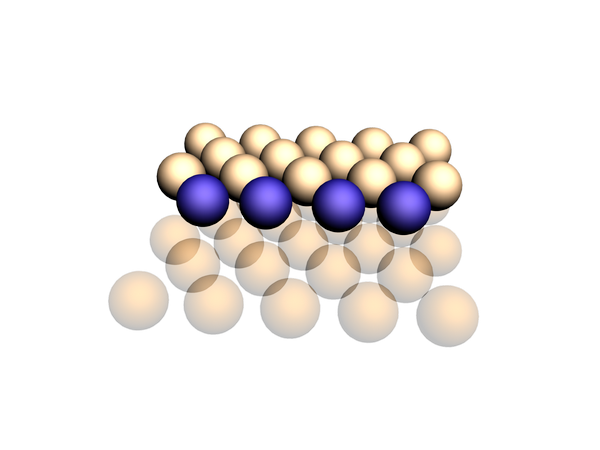
\includegraphics[width=0.25\linewidth]{fig/spt/none.png}};
	\node at (130,0.65) {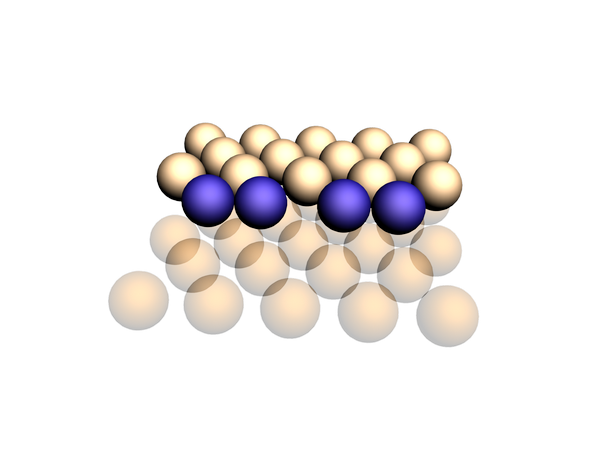
\includegraphics[width=0.25\linewidth]{fig/spt/dipoles-noarrows.png}};
	
	\addplot table[x=T,y=e4]{\Letas};
	\addplot table[x=T,y=e10]{\Letas};
	\addplot table[x=T,y=e16]{\Letas};
	\addplot table[x=T,y=e64]{\Letas};
	
	\draw[thin,tabred,dashed] (225,0) -- ++(0,1);
	\end{axis}
	
	\begin{axis}[
	name=D, at=(C.south), anchor=north, yshift=-0.2cm,
	yticklabels=\empty, xmax=400, ymax=0.032,
	xlabel={$T$, К},
	cycle list={tabblue,tabgreen,taborange,tabred},
	legend style={name=legD},
	]
	\addplot table[x=T,y=de4]{\Ldetas}; \addlegendentry{4 мэВ};
	\addplot table[x=T,y=de10]{\Ldetas}; \addlegendentry{10 мэВ};
	\addplot table[x=T,y=de16]{\Ldetas}; \addlegendentry{16 мэВ};
	\addplot table[x=T,y=de64]{\Ldetas}; \addlegendentry{64 мэВ};
	
	\draw[thin,tabred,dashed] (225,0) -- ++(0,0.04);
	\end{axis}
	
	\tikzset{tag/.style={below left=0.5cm}}
	\node[tag] at (A.north east) {а};
	\node[tag] at (B.north east) {б};
	\node[tag] at (C.north east) {в};
	\node[tag] at (D.north east) {г};
	
	\node[above left] at (legB.north east) {Длина цепочки};
	\node[above left] at (legD.north east) {$\Delta E$};
	\end{tikzpicture}
	\caption{Зависимости параметра порядка $\eta$ и его производной по температуре с обратным знаком $-\od{\eta}{T}$ от температуры для (а, б) цепочек различной длины с $\Delta E=10$~мэВ и (в, г) цепочек длиной 64 атома с разными значениями энергии димеризации $\Delta E$. Подписи к кривым общие для графиков (а) и (б), и (в) и (г).
	Вертикальная пунктирная линия на рисунках (в, г) соответствует температуре структурного фазового перехода для цепочки длиной 64 атома с $\Delta E = 64$~мэВ. Для наглядности слева и справа от нее на рисунке (в) схематически нарисована цепочка до и после структурного фазового перехода.
	}
	\label{fig:etasv2}
\end{figure}


\renewcommand{\chaptermark}[1]{\markboth{\scshape\truncate{0.5\linewidth}{#1}}{}}

% Основные результаты и выводы
\chapter*{Основные результаты и выводы}
\addcontentsline{toc}{chapter}{Основные результаты и выводы}
\chaptermark{Основные результаты и выводы}
\label{chap:conclusion}

\begin{enumerate}
	\item \lipsum[1]

	\item \lipsum[2]

	\item \lipsum[3]

	\item \lipsum[4]

	\item \lipsum[5]

	\item \lipsum[6]
\end{enumerate}


% Список обозначений
%\input{acronyms}

% Списки литературы
% !TeX root = phd_thesis_Syromyatnikov.tex

\chapter*{Литература}
\addcontentsline{toc}{chapter}{Литература}
\chaptermark{Литература}

\printbibliography[heading={none},notkeyword={ownarticle},notkeyword={ownconference}]




\chapter*{Список опубликованных работ}
\addcontentsline{toc}{chapter}{Список опубликованных работ}
\chaptermark{Список опубликованных работ}

\begin{refsection}
\nocite{%
	Syro-JMMM-2020,
	Syromyatnikov2020SurfSci,
	SyromyatnikovMagLett2019,
	SyromyatnikovJetpl2019rus,
	Syromyatnikov:jetp-letters-rus:2018,
	Syromyatnikov:PhysRevB:2018,
	Syromyatnikov:jetp-rus:2017,
	Syromyatnikov:matlet:2016,
	Syromyatnikov:mplb:2016,
	Syromyatnikov:jetp-letters-rus:2014}

\section*{Статьи в научных журналах}
\addcontentsline{toc}{section}{Статьи в научных журналах}
\newrefcontext[labelprefix=A,sorting=none]
\printbibliography[heading={none},resetnumbers=true,keyword={ownarticle}]
\end{refsection}


\begin{refsection}
\nocite{%
	Syromyatnikov:CHPH-WI:2020,
	Klavsyuk2019IWMW,
	klavsyuk2019IBCM,
	Syromyatnikov2019IBCM,
	Syromyatnikov:CHPH-WI:2018,
	Syromyatnikov:ICNT:2018,
	Syromyatnikov:CHPH-WI:2017,
	Syromyatnikov:Lomo-rus:2016,
	Syromyatnikov:ECOSS32,
	Syromyatnikov:Lomo-rus:2015,
	Syromyatnikov:ECOSS30}

\section*{Публикации в сборниках тезисов конференций}
\addcontentsline{toc}{section}{Публикации в сборниках тезисов конференций}
\newrefcontext[labelprefix=T,sorting=none]
\printbibliography[heading={none},resetnumbers=true,keyword={ownconference}]
\end{refsection}

\chapter*{Благодарности}
%\addcontentsline{toc}{chapter}{Благодарности}
\label{chap:ack}

\lipsum[13]

\vspace*{1.5cm}

Работа выполнена при  финансовой поддержке \dots. 

\vfill\hfill{\tiny \textcolor{black!20!white}{\texttt{\GitDescribe}}}


\end{document}
